%% Volkov24fsetV.tex
%% derived from Laporta17figuragauShort.tex %%%%%
%% compiled by  reducesymm/QFT/blog.tex
%% Volkov24fsetV.pdf started as Volkov24 arXiv a1_5loops.ps
%%%%%%%%%%%%%%%%%%%%%%%%%%%%%%%%%%%%%%%%
\begin{figure}[t]
\begin{center}
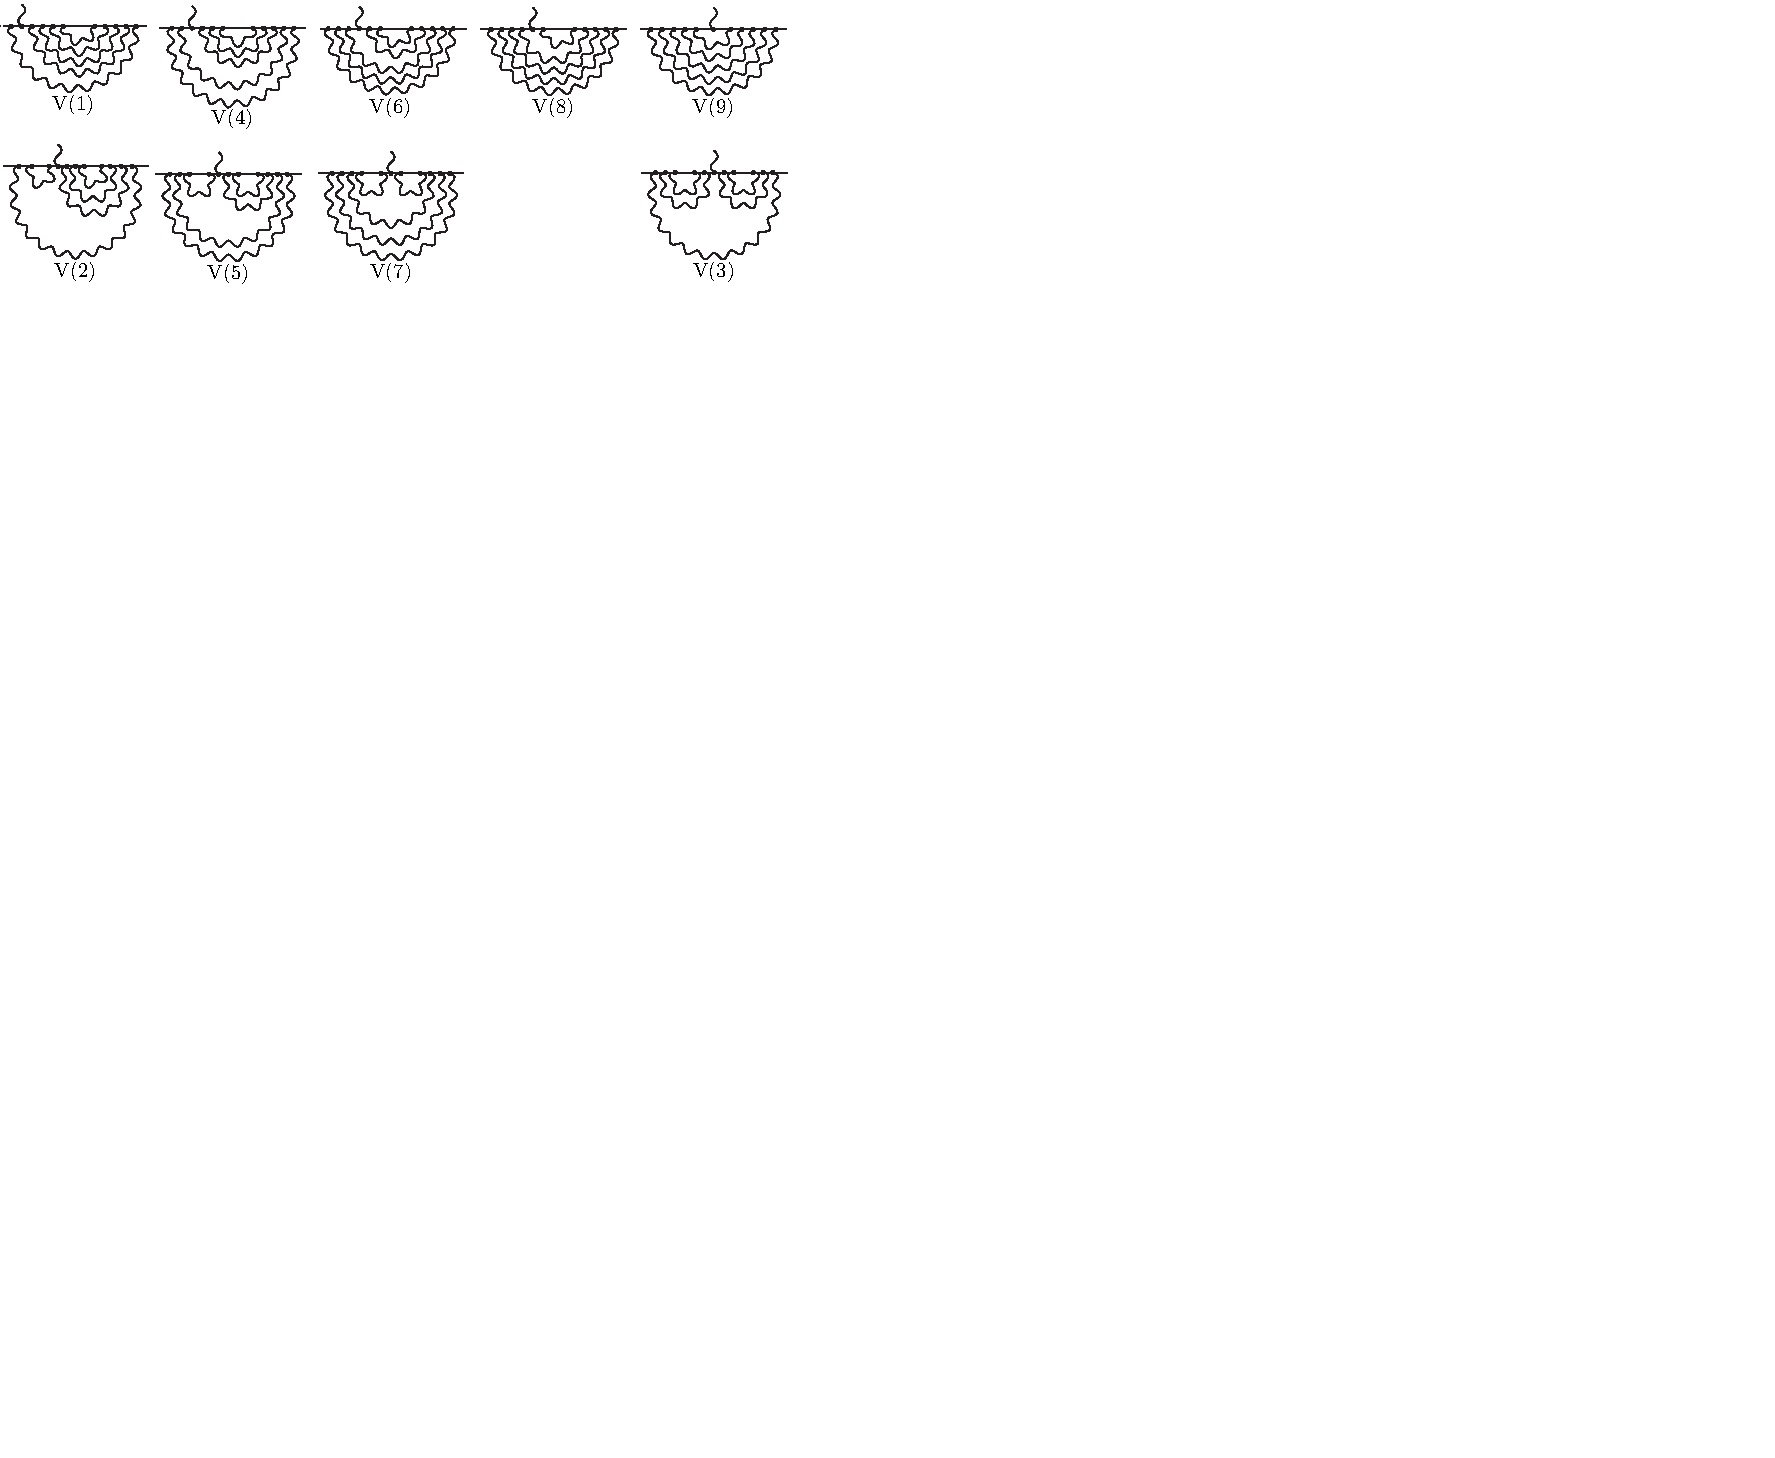
\includegraphics[width=0.9\textwidth]{Volkov24fsetV}
  \\[3ex]
\begin{tabular}{ccrrr}
gauge set &$(k,m,m)$& value~~ & ansatz \\
\hline
  V(1)  & (1,4,0) &   \phantom{+} 6.17  & \phantom{+} 1/2  \\%01
  V(4)  & (2,3,0) &  - 0.80  & - 1/2 \\ %&~(!)\\%02
  V(6)  & (3,2,0) &{\color{red}- 0.41} & \phantom{+} 1/2  \\%03
  V(8)  & (4,1,0) &  - 0.97  & - 1/2  \\%04
  V(9)  & (5,0,0) &  \phantom{+} 1.08  & \phantom{+} 1/2  \\%05
  V(2)  & (1,3,1) &  \phantom{+} 0.96  & \phantom{+} 1/2  \\%06
  V(5)  & (2,2,1) &  - 2.16  &  - 1/2  \\%06
  V(7)  & (3,1,1) &  \phantom{+} 2.64  & \phantom{+} 1/2  \\%06
  V(3)  & (1,2,2) &  \phantom{+} 0.33 & \phantom{+} 1/2  \\%06
\hline
\end{tabular}
 \end{center}
%%/ \phantom{ }\vspace{0truecm}\phantom{ }
\caption{\label{Volkov24fsetV}
5-loop vertex diagrams quenched gauge sets.
% (1)  & (1,4,0)
% (2)  & (1,3,1)
% (3)  & (1,2,2)
% (4)  & (2,3,0)
% (5)  & (2,2,1)
% (6)  & (3,2,0)
% (7)  & (3,1,1)
% (8)  & (4,1,0)
% (9)  & (5,0,0)
The 5-loop gauge-set contributions $a^{(10)}_{kmm'}$, as reported by 
Volkov\rf{Volkov19,Volkov19b,Volkov24}. 
The last column: 1977 Cvitanovi\'c 
predictions\rf{Cvit77b}. Signs are right, except for the set (6) = 
$(3,2,0)$, as is the case for similar 4-loop gauge set (2) = $(2,2,0)$ in 
\reffig{Laporta17figuragauShort}. The remaining sets are close to 
multiples of 1/2, indicated in \reftab{tabGaugeSets}. 
}
 \end{figure}
%%%%%%%%%%%%%%%%%%%%%%%%%%%%%%%%%%%%%%%%
